%\begin{appendices}

\appendix
%\chapter*{ANEXOS}% If \appendix doesn't insert a \chapter
%\addcontentsline{toc}{chapter}{ANEXOS}% Print Appendix in ToC
\setcounter{section}{0}% Reset numbering for sections
\renewcommand{\thesection}{\Alph{section}}% Adjust section printing (from here onward)
	
	
	%\chapter*{Árbol de Problemas}
	%\addcontentsline{toc}{section}{Árbol de Problemas}
	%\renewcommand{\thechapter}{A}
	\label{anexo1}
	\begin{landscape}
		\section{Árbol de Problemas}
		\begin{figure}[H]
			\centering
			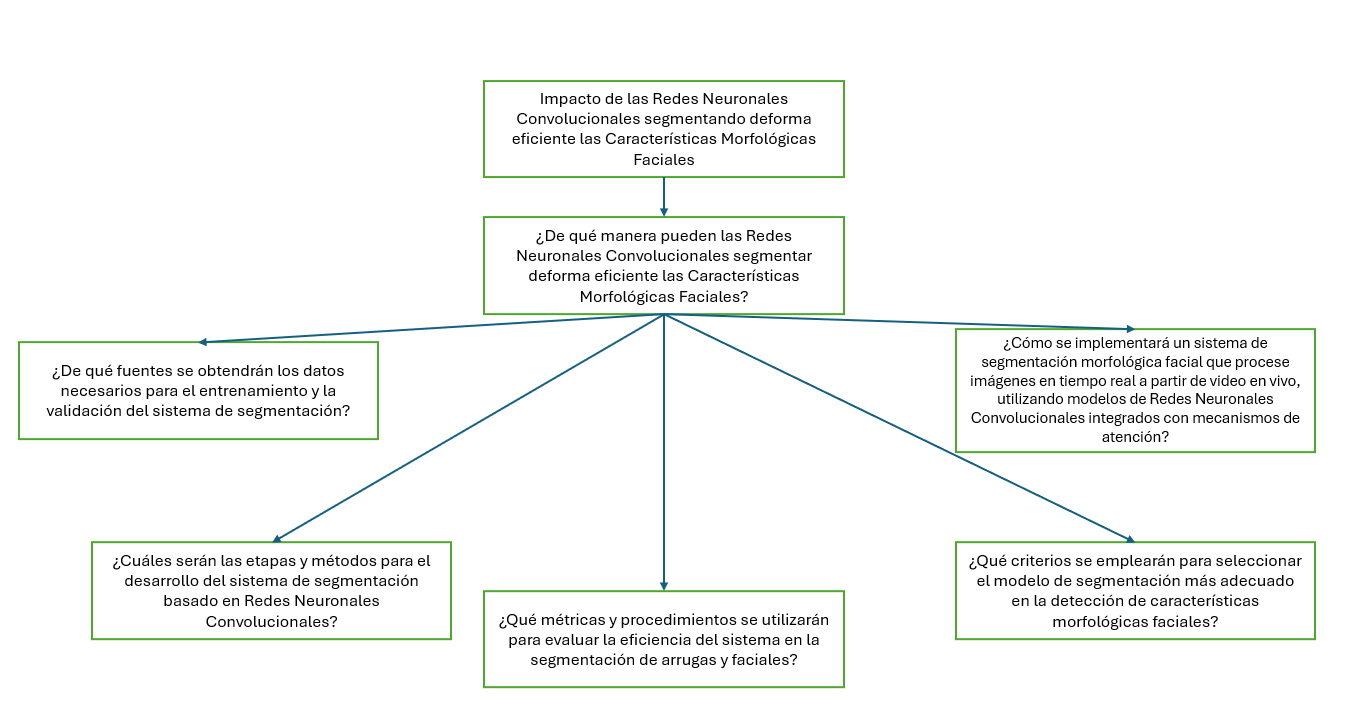
\includegraphics[width=\linewidth]{anexos/arb_problemas.jpg}
			%\caption{Fuente: Elaboración propia}
		\end{figure}
		\end{landscape}
	\clearpage
	
	
	%\chapter*{Árbol de Objetivos}
	%\addcontentsline{toc}{section}{Árbol de Objetivos}
	%\renewcommand{\thechapter}{A}
	\label{anexo2}
	\begin{landscape}
		\section{Árbol de Objetivos}
	\begin{figure}[H]
		\centering
			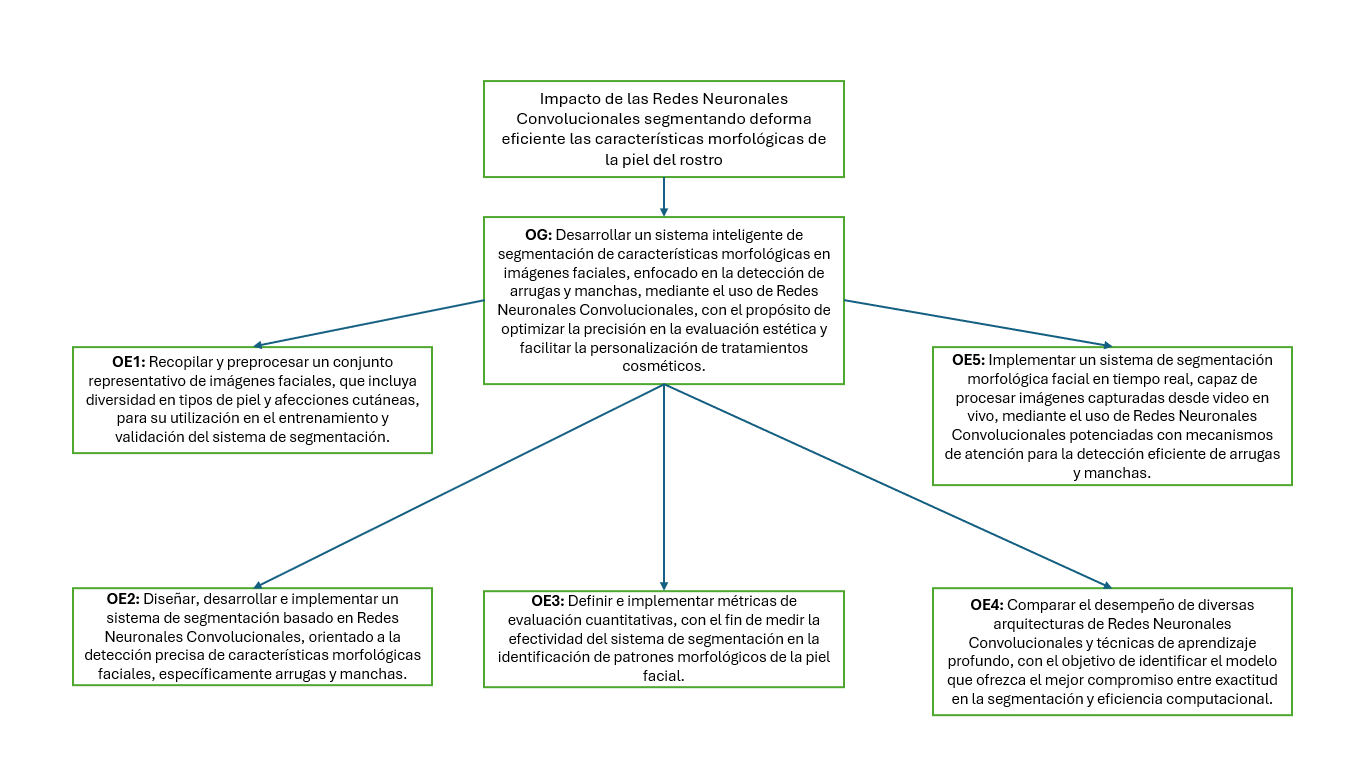
\includegraphics[width=\linewidth]{anexos/arb_objetivos.jpg}
			%\caption{Fuente: Elaboración propia}
	\end{figure}
	\end{landscape}
	\clearpage
	

	\begin{landscape}
		\section{Matriz de Consistencia}
		\label{anexo3}
		\begin{longtable}{ p{3.5cm}p{3.5cm}p{3.5cm}p{3cm}p{3cm}p{3cm}p{3cm} }
			%\centering
			\small
			\tabularnewline \specialrule{.1em}{.05em}{.05em}
			\centering{Título de la tesis} & \multicolumn{6}{p{19cm}}{Segmentación Avanzada de Características Morfológicas Faciales usando Redes Neuronales Convolucionales: Enfoque en Arrugas y Manchas}
			\tabularnewline \specialrule{.1em}{.05em}{.05em}
			\Centering{Problema General}& \Centering{Objetivo General}& \Centering{Hipótesis General}& \Centering{Variables}& \Centering{Dimensiones}& \Centering{Indicadores}& \Centering{Metodología}
			\\
			\specialrule{.1em}{.05em}{.05em}
			{\ProblemaGeneral} & { \ObjetivoGeneral} & {\HipotesisGeneral}
			& \multirow{3}{3cm}[-28ex]{
				\centering Independiente: Imágenes con Características Morfológicas Faciales (Arrugas y Manchas)
			}
			& \multirow{2}{3cm}[-30ex]{
				\centering Modelo de Segmentación Avanzada de las Características Morfológicas Faciales
			}
			& \multirow{1}{3cm}[-10ex]{
				\centering Cantidad de modelos de Segmentación Avanzada
			}
			& \multirow{2}{3cm}[3ex]{
			\setlist{nolistsep}
			\begin{itemize}[label={--},nosep,noitemsep,leftmargin=*,topsep=0pt,partopsep=0pt]
				\item Tipo de investigación: Diseño Experimental.
				\item Alcance de la investigación: Explicativo.
				\item Enfoque de investigación: Cuantitativa.
			\end{itemize}
			}
			\\
			\cline{1-3}
			\cline{6-6}
			\Centering{Problemas Específicos}& \Centering{Objetivos Específicos} & \Centering{Hipótesis Específicas}
			& 
			&
			& \multirow{1}{3cm}[-10ex]{
				\centering Efectividad de modelos de Segmentación Avanzada
			}
			& 
			\\
			\cline{1-3}
			\vspace{0pt}{\Pbone} & \vspace{0pt}{\Objone} & \vspace{0pt}{\Hone} &  &  &  &
			\\
			\cline{1-3}
			\cline{5-6}
			\vspace{0pt}{\Pbtwo} & \vspace{0pt}{\Objtwo} & \vspace{0pt}{\Htwo} &  & \multirow{2}{3cm}[-15ex]{
				\centering Estructura del modelo de Segmentación Avanzada
			} & \multirow{1}{3cm}[-13ex]{
				\centering Complejidad de la estructura de modelos de Segmentación Avanzada
			} &
			\\
			\cline{1-6}
			\vspace{0pt}{\Pbthree} & \vspace{0pt}{\Objthree} & \vspace{0pt}{\Hthree}
			& \multirow{2}{3cm}[-20ex]{
				\centering Dependiente: Segmentación Avanzada de las Características Morfológicas Faciales
			} 
			& \multirow{1}{3cm}[-10ex]{
				\centering Tipos de Piel
			}
			& \multirow{1}{3cm}[-6.5ex]{
				\centering Características Morfológicas Faciales
			}
			& 
			\\
			\cline{1-3}
			\cline{5-6}
			\vspace{0pt}{\Pbfour} & \vspace{0pt}{\Objfour} & \vspace{0pt}{\Hfour} &  & \multirow{1}{3cm}[-12ex]{
				\centering Desempeño computacional del sistema
			} & \multirow{1}{3.5cm}[-8ex]{
				\setlist{nolistsep}
				\begin{itemize}[label={--},nosep,noitemsep,leftmargin=*,topsep=0pt,partopsep=0pt]
					\item Metainformación.
					\item Descripción.
					\item Comentarios.
				\end{itemize}
				} & 
				\\
				\cline{1-3}
				\cline{5-6}
				\vspace{0pt}{\Pbfive} & \vspace{0pt}{\Objfive} & \vspace{0pt}{\Hfive} & & \multirow{1}{3cm}[-10ex]{
					\centering Implementación del modelo de segmentación con retroalimentación de usuarios
				} & \multirow{1}{3cm}[-8ex]{
					\centering Nivel de satisfacción con los resultados de la segmentación
				} & 
				\\
				\specialrule{.1em}{.05em}{.05em}
				\end{longtable}
				\end{landscape}
				\clearpage

	% \begin{landscape}
	% 	\section{Matriz de Consistencia}
	% 	\label{anexo3}
	% 	\renewcommand{\arraystretch}{1.5} % Espaciado entre filas
	% 	\small % Reducir el tamaño del texto
		
	% 	\begin{longtable}{p{3cm}p{3cm}p{3cm}p{2.5cm}p{2.5cm}p{2.5cm}p{2.5cm}}
	% 	\hline
	% 	\multicolumn{7}{c}{\textbf{Título de la tesis:} Segmentación Avanzada de Características Morfológicas Faciales usando Redes Neuronales Convolucionales: Enfoque en Arrugas y Manchas} \\
	% 	\hline
	% 	\textbf{Problema General} & \textbf{Objetivo General} & \textbf{Hipótesis General} & \textbf{Variable Dependiente} & \textbf{Variable Independiente} & \textbf{Método} & \textbf{Alcance} \\
	% 	\hline
	% 	{\ProblemaGeneral} & {\ObjetivoGeneral} & {\HipotesisGeneral} &
	% 	Eficiencia en la Segmentación de Características Faciales &
	% 	Aplicación de Redes Neuronales Convolucionales &
	% 	\multirow{6}{2.5cm}{\centering Tipo de Investigación: Experimental} &
	% 	\multirow{6}{2.5cm}{\centering Alcance: Explicativo} \\
	% 	\cline{1-5}
	% 	\textbf{Problemas Específicos} & \textbf{Objetivos Específicos} & \textbf{Hipótesis Específicas} & \textbf{Dependiente} & \textbf{Independiente} & & \\
	% 	\cline{1-5}
	% 	{\Pbone} & {\Objone} & {\Hone} &
	% 	Conjunto de Imágenes Representativo y Preprocesado &
	% 	Imágenes Faciales & & \\
	% 	\cline{1-5}
	% 	{\Pbtwo} & {\Objtwo} & {\Htwo} &
	% 	Precisión en la Detección de Características Faciales &
	% 	Sistema de Segmentación CNN & & \\
	% 	\cline{1-5}
	% 	{\Pbthree} & {\Objthree} & {\Hthree} &
	% 	Efectividad del Sistema en Patrones Faciales &
	% 	Métricas de Evaluación Cuantitativas & & \\
	% 	\cline{1-5}
	% 	{\Pbfour} & {\Objfour} & {\Hfour} &
	% 	Exactitud y Eficiencia Computacional &
	% 	Arquitecturas CNN y Deep Learning & & \\
	% 	\cline{1-5}
	% 	{\Pbfive} & {\Objfive} & {\Hfive} &
	% 	Eficiencia en la Detección de Arrugas y Manchas &
	% 	Sistema CNN con Atención & & \\
	% 	\hline
	% 	\end{longtable}
	% 	\end{landscape}
	% 	\clearpage
		